% Methodology section
Modeling temporality is central to be able to capture the true essence of complex systems. Components of complex systems interact with one another and evolve across multiple time scales, leading to emergent phenomena that cannot be understood through static or purely structural models. However for modeling such systems, it is sufficient to model the participant components and their interactions as stochastic processes that evolve over time, rather than modeling time explicitly. This implies our model must capture sequences that represent the evolution of states and interactions over time, while preserving causal relationships. The different scales of time are captured by the hierarchical structure of operads, where different levels of the hierarchy can represent dynamics occurring at different time scales, with higher levels operating at slower time scales than lower ones.

We develop a novel mathematical framework, based on WD-operads, to model complex systems through temporal-causal relationships. Our approach enriches the established theory of WD-operads with temporal probability structures, creating operads that naturally capture sequential dynamics and causal interactions.

\subsection{Temporal Probability Spaces}

Let us first define the notion of temporal probability spaces, which will serve as an enriching category for our operads. We denote the category of temporal probability spaces as $\mathbf{TempProb}$, a subcategory of $\mathbf{Stoch}$ (or $\mathbf{Meas}$) specifically designed to enforce temporal causality through filtrations.

Each object of $\mathbf{TempProb}$ is a temporal probability space, $\Omega_{\mathcal{W}}$, shortened as $\Omega$, where each object of the space represents a state of the system at a given time. Hence for each box of the WD-operad $\mathcal{W}$, the space $\Omega_{\mathcal{W}}$ contains the set of all possible execution paths or histories of the system component represented by that box. Additionally, to enable us to assign probabilities to subsets of these execution paths, we equip each temporal probability space with a sigma-algebra $\mathcal{F}$ of measurable events and a probability measure $\mathbb{P}$ that assigns probabilities to these events.

Morphisms in $\mathbf{TempProb}$ are stochastic kernels that preserve the temporal structure of the spaces, ensuring that information flows consistently through time. A morphism between two temporal probability spaces represents how the probabilistic evolution of one system component conditions or influences the probability distribution over possible evolutions of another component over time. For example, a morphism $K: \Omega_{\mathcal{W}_1} \to \Omega_{\mathcal{W}_2}$ between two temporal probability spaces can be viewed as a stochastic kernel that maps each execution path in $\Omega_{\mathcal{W}_1}$ to a probability distribution over execution paths in $\Omega_{\mathcal{W}_2}$, while respecting the temporal ordering of events. At time $t$, given history up to time $t$ in $\Omega_{\mathcal{W}_1}$, the morphism $K$ tells us the conditional probability distribution over possible states at time $t$ in $\Omega_{\mathcal{W}_2}$.

Formally, the category $\mathbf{TempProb}$ is defined as follows:

\begin{itemize}
    \item \textbf{Objects}: Temporal probability spaces $(\Omega, \mathcal{F}, \{\mathcal{F}_t\}_{t \geq 0}, \mathbb{P})$ where:
    \begin{itemize}
        \item $\Omega$ is the sample space, representing the set of all possible system trajectories or execution paths.
        \item $\mathcal{F}$ is a sigma-algebra on $\Omega$ - the collection of measurable events (subsets of trajectories) to which we can assign probabilities. Not every arbitrary subset of $\Omega$ is measurable; $\mathcal{F}$ specifies which subsets are "well-behaved" enough for probability theory.
        \item $\{\mathcal{F}_t\}_{t \geq 0}$ is a filtration - an increasing family of sigma-algebras where $\mathcal{F}_s \subseteq \mathcal{F}_t$ for $s \leq t$. This represents the accumulation of information: $\mathcal{F}_t$ captures everything we can know about the system's history up to time $t$.
        \item $\mathbb{P}: \mathcal{F} \to [0,1]$ is a probability measure assigning a likelihood to each measurable event.
    \end{itemize}

    \item \textbf{Morphisms}: Stochastic kernels $K: (\Omega_1, \mathcal{F}_1, \{\mathcal{F}_t^1\}) \to (\Omega_2, \mathcal{F}_2, \{\mathcal{F}_t^2\})$ that are adapted to the filtrations. These represent how one system component probabilistically influences another while respecting causality: at each time $t$, $K$ maps histories in $\Omega_1$ (measurable with respect to $\mathcal{F}_t^1$) to probability distributions over histories in $\Omega_2$. Formally, $K_t$ is $\mathcal{F}_t^1$-measurable for all $t$, ensuring the influence cannot depend on future information.

    \item \textbf{Composition}: Temporal probability spaces compose via a 2-step process:

    \textbf{Step 1 - Monoidal product}: For any two spaces, we first form the product:
    \[(\Omega_1, \mathcal{F}_1, \{\mathcal{F}_t^1\}, \mathbb{P}_1) \otimes (\Omega_2, \mathcal{F}_2, \{\mathcal{F}_t^2\}, \mathbb{P}_2) = (\Omega_1 \times \Omega_2, \mathcal{F}_1 \otimes \mathcal{F}_2, \mathcal{F}_t^1 \otimes \mathcal{F}_t^2, \mathbb{P}_1 \times \mathbb{P}_2)\]

    \textbf{Step 2 - Dependency modification}: For dependent systems, stochastic kernels $K: \Omega_1 \to \Omega_2$ modify the joint probability measure on the product space to create causal dependencies. Multiple dependencies compose via the Chapman-Kolmogorov equation \citep{kadanoff2000statistical}:
    \[(L \circ K)(\omega_1, A) = \int_{\Omega_2} K(\omega_1, d\omega_2) L(\omega_2, A)\]
\end{itemize}

This category captures the essential features of complex systems: information accumulates through time (filtration), future states depend probabilistically on past states (stochastic kernels), temporal ordering enforces causality (adaptedness), and independent subsystems can evolve in parallel (monoidal structure).

\subsubsection{Example: Neural Spike Chains}

As a concrete example of $\mathbf{TempProb}$, consider a simple system with two neurons arranged in sequence:

\[(input) \xrightarrow{} [neuron_1] \xrightarrow{} [neuron_2] \xrightarrow{} (output)\]

Each neuron fires with a stochastic spike when its input exceeds a certain threshold, with some probability. For an input voltage of $x$ volts, the sample space $\Omega$ contains all conceivable sequences, including acausal ones like backwards information flow. However, we focus on the $\sigma$-algebra $\mathcal{F}$ which contains only measurable events - causally valid sequences that respect temporal ordering.

Examples of events in $\mathcal{F}$ include:
\begin{itemize}
    \item $\omega_0$: $(input = x)$ only (initial state)
    \item $\omega_1$: $(input = x) \to [neuron_1 \text{ fires at } t_1]$
    \item $\omega_2$: $(input = x) \to [neuron_1 \text{ does not fire}]$
    \item $\omega_3$: $(input = x) \leftarrow [neuron_1 \text{ fires at } t_1]$ (absurd)
    \item $\omega_4$: $(input = x) \to [neuron_1 \text{ fires at } t_1] \to [neuron_2 \text{ does not fire}]$
    \item $\omega_5$: $(input = x) \to [neuron_1 \text{ fires at } t_2] \leftarrow [neuron_2 \text{ fires at } t_1]$ (absurd)
    \item $\omega_6$: $(input = x) \leftarrow [neuron_1 \text{ fires at } t_2] \to [neuron_2 \text{ fires at } t_1]$ (absurd)
    \item $\omega_7$: $(input = x) \to [neuron_1 \text{ fires at } t_1] \to [neuron_2 \text{ fires at } t_2] \to (output)$
    \item etc.
\end{itemize}

Note that the internal dynamics of each neuron are abstracted away; we focus on observable spike events and their temporal ordering. The $\sigma$-algebra $\mathcal{F}$ excludes acausal sequences like $(input) \leftarrow [neuron_1] \leftarrow [neuron_2]$ - while these might exist in $\Omega$, they are not measurable events in $\mathcal{F}$.

The filtration $\{\mathcal{F}_t\}_{t > 0}$ captures information accumulation:
\begin{itemize}
    \item $\mathcal{F}_{t_1}$: Events knowable up to $t_1$ (input + neuron1 state)
    \item $\mathcal{F}_{t_2}$: Events knowable up to $t_2$ (full system state, including output)
\end{itemize}

Each event has an associated probability:
\begin{align}
\mathbb{P}(\omega_1) &= P(\text{neuron}_1 \text{ fires} \mid \text{input} = x) \\
\mathbb{P}(\omega_7) &= P(\text{neuron}_1 \text{ fires} \mid x) \cdot P(\text{neuron}_2 \text{ fires} \mid \text{neuron}_1 \text{ fired})
\end{align}

\subsubsection{Example: Composition of two spaces}

Now, we show how temporal probability spaces compose. For simplicity, let's decompose our neural chain in the previous example into two separate TempProb objects and see how they combine.

\textbf{First component:} $(\Omega^1, \mathcal{F}^1, \{\mathcal{F}_t^1\}, \mathbb{P}^1)$ represents (input) → [neuron$_1$] → (output) system:
\begin{itemize}
    \item $\Omega^1$ contains all conceivable sequences: input → neuron$_1$ → output
    \item $\mathcal{F}^1$ contains measurable events like: $(input)$, $(input) \to [neuron_1 \text{ fires}] \to (output)$, $(input) \to [neuron_1 \text{ does not fire}]$ with $\{\mathcal{F}_1^1\}$ capturing information at $t_1$
    \item $\mathbb{P}^1$ assigns probabilities to events in $\mathcal{F}_1^1$
\end{itemize}

\textbf{Second component:} $(\Omega^2, \mathcal{F}^2, \{\mathcal{F}_t^2\}, \mathbb{P}^2)$ represents a separate (input) → [neuron$_2$] → (output) system:
\begin{itemize}
    \item $\Omega^2$ contains all conceivable sequences: input → neuron$_2$ → output
    \item $\mathcal{F}^2$ contains measurable events like: $(input)$, $(input) \to [neuron_2 \text{ fires}] \to (output)$, $(input) \to [neuron_2 \text{ does not fire}]$ with $\{\mathcal{F}_1^2\}$ capturing information at $t_1$
    \item $\mathbb{P}^2$ assigns probabilities to events in $\mathcal{F}_1^2$
\end{itemize}

We compose temporal probability spaces in two steps:

\textbf{Step 1 - Monoidal product:} We first combine the systems using the monoidal structure:
\[(\Omega^1, \mathcal{F}^1, \{\mathcal{F}_t^1\}, \mathbb{P}^1) \otimes (\Omega^2, \mathcal{F}^2, \{\mathcal{F}_t^2\}, \mathbb{P}^2) = (\Omega^1 \times \Omega^2, \mathcal{F}^1 \otimes \mathcal{F}^2, \mathcal{F}_t^1 \otimes \mathcal{F}_t^2, \mathbb{P}^1 \times \mathbb{P}^2)\]

\textbf{Step 2 - Add dependencies (if needed):} For independent systems, we stop at Step 1. For dependent systems, we apply stochastic kernels to modify the probability measure on the product space. A kernel $K: \Omega^1 \to \Omega^2$ creates dependencies by changing the joint distribution:
\[
\mathbb{P}(\text{dependent})(\omega_1, \omega_2) = \mathbb{P}^1(\omega_1) \cdot K(\omega_1, \omega_2)
\]
where the Chapman-Kolmogorov equation ensures consistent composition of multiple dependencies.

\subsubsection{Example: Temporal Integration with Delays}

Consider a more complex scenario where $neuron_2$ receives two inputs: one from neuron$_1$ and a delayed external input $input_2$. Suppose $neuron_2$ has a memory window and can integrate signals arriving at different times. Lets model the second component from above again:

The temporal probability space $(\Omega^2, \mathcal{F}^2, \{\mathcal{F}_t^2\}, \mathbb{P}^2)$ for this system contains paths like:
\begin{itemize}
    \item $\omega_1$: $(input_1), (input_2) \to [neuron_2 \text{ fires}] \to output$
    \item $\omega_2$: $(input_1), (input_2) \to [neuron_2 \text{ does not fire}]$
\end{itemize}

The filtration captures the accumulation of temporal information:
\begin{itemize}
    \item $\mathcal{F}_{t_1}^2$: Information about $\text{neuron}_2$ firing after $input_1$ has arrived
    \item $\mathcal{F}_{t_2}^2$: Information about $\text{neuron}_2$ firing after $input_2$ has arrived
    \item The probability depends on delay: $\mathbb{P}(\text{neuron}_2 \text{ fires} \mid \text{both inputs, delay } \delta)$ where $\delta = |t_2 - t_1|$
\end{itemize}

The insight here is that the temporal probability structure is fundamentally event-based rather than clock-time-based:
\begin{itemize}
    \item \textbf{Events, not times}: The model tracks which events happened and their causal ordering, not precise timestamps. $neuron_2$ fires after $neuron_1$.
    \item \textbf{Delay as probability parameter}: The actual delay $\delta$ doesn't change the structure of $\Omega$ or $\mathcal{F}$ - it only affects $\mathbb{P}$, or the delay is a parameter to calculate the probability. Short delays might give $\mathbb{P}(\text{fire}) = 0.9$, long delays $\mathbb{P}(\text{fire}) = 0.1$.
    \item \textbf{Conditional dependencies}: What matters is whether neuron$_1$ fired (and when relative to other events), not the absolute timestamp. The filtration $\mathcal{F}_t$ captures what events have occurred rather than what time is it.
\end{itemize}

\subsection{$\mathcal{S}$-operads: TempProb-Enriched WD-Operads}

We now define $\sigma$-operads as WD-operads enriched in $\mathbf{TempProb}$. Let $\mathcal{W}$ be the standard operad of wiring diagrams with interfaces (finite sets of typed ports) as objects and wiring diagrams as morphisms.

A $\sigma$-operad $\mathcal{W}_{\sigma}$ is the $\mathbf{TempProb}$-enrichment of $\mathcal{W}$, where:
\begin{itemize}
    \item \textbf{Objects}: Same as $\mathcal{W}$ - interfaces representing system boundaries.
    \item \textbf{Hom-objects}: $\mathcal{W}_{\sigma}(X,Y)$ is a temporal probability space rather than a set. Each wiring diagram now carries probabilistic temporal dynamics.
    \item \textbf{Composition}: Follows the 2-step TempProb composition: first monoidal product (for independent systems), then dependency modification via stochastic kernels (for connected ports).
\end{itemize}

\begin{figure}[ht]
\centering
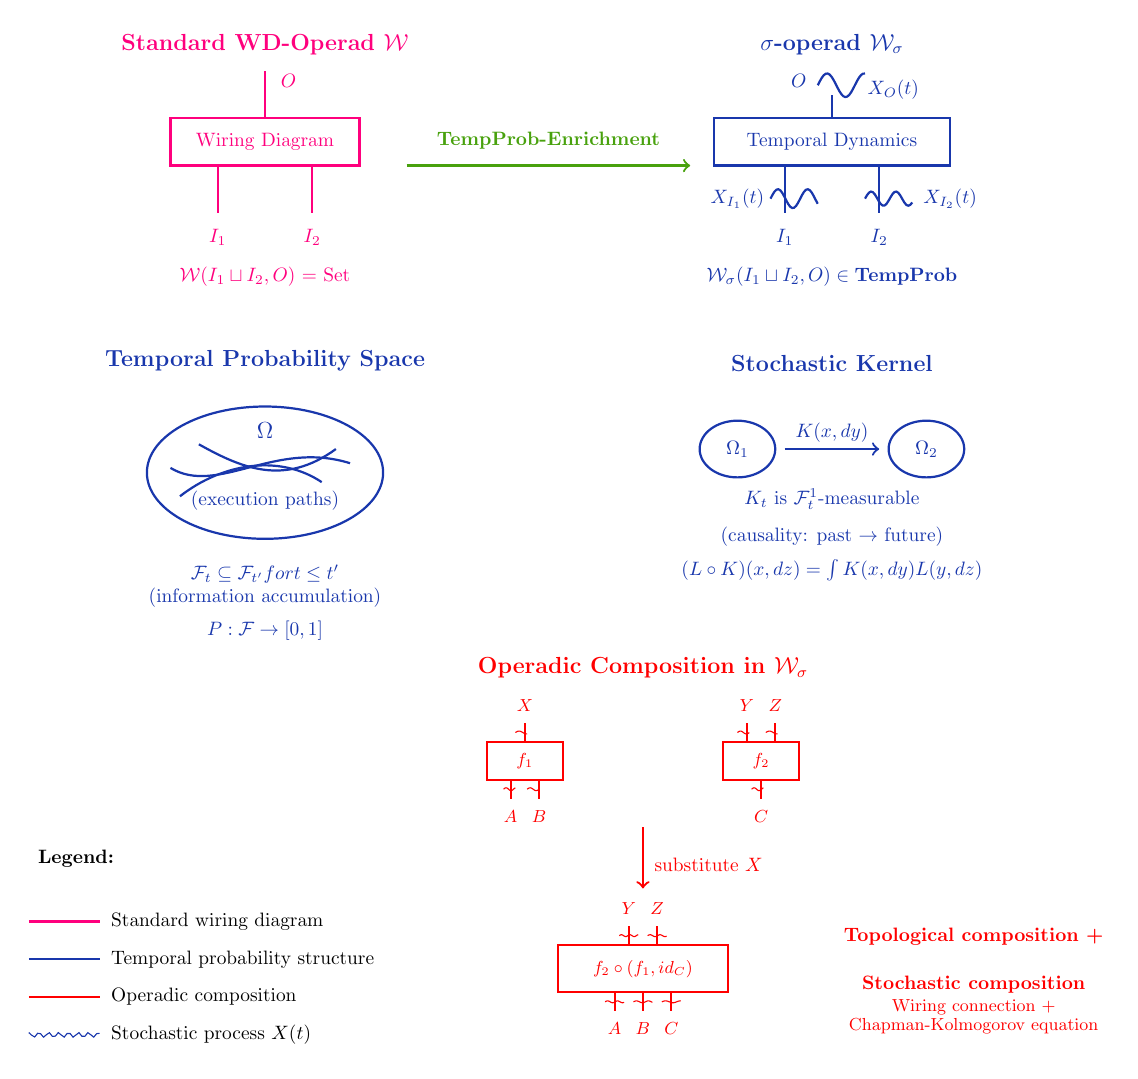
\begin{tikzpicture}[scale=0.6, every node/.style={scale=0.7}]

% Define colors - High Contrast Professional Palette
\definecolor{wdcolor}{RGB}{255, 0, 125}
\definecolor{tempcolor}{RGB}{25, 55, 172}
\definecolor{enrichcolor}{RGB}{72, 161, 13}
\definecolor{compcolor}{RGB}{255, 0, 0}

% Title
% \node[above] at (0, 8) {\Large\textbf{$\sigma$-operads: TempProb-Enriched Wiring Diagrams}};

% Part 1: Standard Wiring Diagram (left side)
\begin{scope}[shift={(-6, 4)}]
    \node[above, wdcolor, font=\large] at (0, 2.2) {\textbf{Standard WD-Operad $\mathcal{W}$}};

    % Input interfaces
    \draw[thick, wdcolor] (-1, -1) -- (-1, 0);
    \draw[thick, wdcolor] (1, -1) -- (1, 0);
    \node[below, wdcolor] at (-1, -1.2) {$I_1$};
    \node[below, wdcolor] at (1, -1.2) {$I_2$};

    % Box
    \draw[thick, wdcolor] (-2, 0) rectangle (2, 1);
    \node[wdcolor] at (0, 0.5) {Wiring Diagram};

    % Output interface
    \draw[thick, wdcolor] (0, 1) -- (0, 2);
    \node[above, wdcolor] at (0.5, 1.5) {$O$};

    % Hom-set notation
    \node[below, wdcolor] at (0, -2) {$\mathcal{W}(I_1 \sqcup I_2, O)$ = Set};
\end{scope}

% Arrow indicating enrichment
\draw[->, thick, enrichcolor] (-3, 4) -- (3, 4);
\node[above, enrichcolor] at (0, 4.2) {\textbf{TempProb-Enrichment}};

% Part 2: Temporal Probability Enriched (right side)
\begin{scope}[shift={(6, 4)}]
    \node[above, tempcolor, font=\large] at (0, 2.2) {\textbf{$\sigma$-operad $\mathcal{W}_\sigma$}};

    % Input interfaces with temporal processes
    \draw[thick, tempcolor] (-1, -1) -- (-1, 0);
    \draw[thick, tempcolor] (1, -1) -- (1, 0);
    \node[below, tempcolor] at (-1, -1.2) {$I_1$};
    \node[below, tempcolor] at (1, -1.2) {$I_2$};

    % Temporal processes at inputs
    \draw[tempcolor, thick, domain=0:1] plot (\x-1.3, {0.2*sin(10*\x r) - 0.7});
    \draw[tempcolor, thick, domain=0:1] plot (\x+0.7, {0.15*sin(12*\x r) - 0.7});
    \node[tempcolor] at (-2, -0.7) {$X_{I_1}(t)$};
    \node[tempcolor] at (2.5, -0.7) {$X_{I_2}(t)$};

    % Box with temporal dynamics
    \draw[thick, tempcolor] (-2.5, 0) rectangle (2.5, 1);
    \node[tempcolor] at (0, 0.5) {Temporal Dynamics};

    % Output with temporal process
    \draw[thick, tempcolor] (0, 1) -- (0, 1.5);
    \node[above, tempcolor] at (-0.7, 1.5) {$O$};
    \draw[tempcolor, thick, domain=0:1] plot (\x-0.3, {0.25*sin(8*\x r) + 1.7});
    \node[tempcolor] at (1.3, 1.6) {$X_O(t)$};

    % Hom-object notation
    \node[below, tempcolor] at (0, -2) {$\mathcal{W}_\sigma(I_1 \sqcup I_2, O) \in \mathbf{TempProb}$};
\end{scope}

% Part 3: Temporal Probability Space Details (middle-left)
\begin{scope}[shift={(-6, -2.5)}]
    \node[above, tempcolor, font=\large] at (0, 2) {\textbf{Temporal Probability Space}};

    % Sample space
    \draw[thick, tempcolor] (0, 0) ellipse (2.5 and 1.4);
    \node[tempcolor, font=\large] at (0, 0.9) {$\Omega$};
    \node[tempcolor] at (0, -0.6) {(execution paths)};

    % Trajectories
    \draw[tempcolor, thick] (-1.8, -0.5) .. controls (-0.9, 0.2) and (0.3, 0.4) .. (1.2, -0.2);
    \draw[tempcolor, thick] (-1.4, 0.6) .. controls (-0.5, 0.1) and (0.4, -0.3) .. (1.5, 0.5);
    \draw[tempcolor, thick] (-2.0, 0.1) .. controls (-1.0, -0.5) and (0.2, 0.7) .. (1.8, 0.2);

    % Filtration
    \node[below, tempcolor] at (0, -1.8) {$\mathcal{F}_t \subseteq \mathcal{F}_{t'} \text{ for } t \leq t'$};
    \node[below, tempcolor] at (0, -2.3) {(information accumulation)};

    % Measure
    \node[below, tempcolor] at (0, -3) {$\mathbb{P}: \mathcal{F} \to [0,1]$};
\end{scope}

% Part 4: Stochastic Kernel (middle-right)
\begin{scope}[shift={(6, -2.5)}]
    \node[above, tempcolor, font=\large] at (0, 2) {\textbf{Stochastic Kernel}};

    % Source space
    \draw[thick, tempcolor] (-2, 0.5) ellipse (0.8 and 0.6);
    \node[tempcolor] at (-2, 0.5) {$\Omega_1$};

    % Target space
    \draw[thick, tempcolor] (2, 0.5) ellipse (0.8 and 0.6);
    \node[tempcolor] at (2, 0.5) {$\Omega_2$};

    % Kernel arrow
    \draw[->, thick, tempcolor] (-1, 0.5) -- (1, 0.5);
    \node[above, tempcolor] at (0, 0.5) {$K(x, dy)$};

    % Adaptedness condition
    \node[below, tempcolor] at (0, -0.2) {$K_t$ is $\mathcal{F}_t^1$-measurable};
    \node[below, tempcolor] at (0, -1) {(causality: past $\to$ future)};

    % Chapman-Kolmogorov
    \node[below, tempcolor] at (0, -1.7) {$(L \circ K)(x, dz) = \int K(x, dy) L(y, dz)$};
\end{scope}

% Part 5: Composition Diagram (bottom)
\begin{scope}[shift={(2, -10)}]
    \node[above, compcolor, font=\large] at (0, 3) {\textbf{Operadic Composition in $\mathcal{W}_\sigma$}};

    % First component
    \begin{scope}[shift={(-2.5, 1)}]
        \draw[thick, compcolor] (-0.8, 0) rectangle (0.8, 0.8);
        \node[compcolor, font=\small] at (0, 0.4) {$f_1$};

        \draw[thick, compcolor] (-0.3, 0) -- (-0.3, -0.4);
        \draw[thick, compcolor] (0.3, 0) -- (0.3, -0.4);
        \node[below, compcolor, font=\small] at (-0.3, -0.5) {$A$};
        \node[below, compcolor, font=\small] at (0.3, -0.5) {$B$};

        \draw[thick, compcolor] (0, 0.8) -- (0, 1.2);
        \node[above, compcolor, font=\small] at (0, 1.3) {$X$};

        % Temporal processes (smaller)
        \draw[compcolor, domain=0:0.25] plot (\x-0.45, {0.03*sin(30*\x r) + -0.2});
        \draw[compcolor, domain=0:0.25] plot (\x+0.05, {0.03*sin(25*\x r) + -0.2});
        \draw[compcolor, domain=0:0.25] plot (\x-0.2, {0.03*sin(20*\x r) + 1.0});
    \end{scope}

    % Second component
    \begin{scope}[shift={(2.5, 1)}]
        \draw[thick, compcolor] (-0.8, 0) rectangle (0.8, 0.8);
        \node[compcolor, font=\small] at (0, 0.4) {$f_2$};

        \draw[thick, compcolor] (0, 0) -- (0, -0.4);
        \node[below, compcolor, font=\small] at (0, -0.5) {$C$};

        \draw[thick, compcolor] (-0.3, 0.8) -- (-0.3, 1.2);
        \draw[thick, compcolor] (0.3, 0.8) -- (0.3, 1.2);
        \node[above, compcolor, font=\small] at (-0.3, 1.3) {$Y$};
        \node[above, compcolor, font=\small] at (0.3, 1.3) {$Z$};

        % Temporal processes (smaller)
        \draw[compcolor, domain=0:0.25] plot (\x-0.2, {0.03*sin(30*\x r) + -0.2});
        \draw[compcolor, domain=0:0.25] plot (\x-0.5, {0.03*sin(25*\x r) + 1.0});
        \draw[compcolor, domain=0:0.25] plot (\x+0.1, {0.03*sin(20*\x r) + 1.0});
    \end{scope}

    % Composition arrow (Vertical now)
    \draw[->, thick, compcolor] (0, 0) -- (0, -1.3);
    \node[right, compcolor] at (0.1, -0.8) {substitute $X$};

    % Composed system
    \begin{scope}[shift={(0, -3.5)}]
        \draw[thick, compcolor] (-1.8, 0) rectangle (1.8, 1);
        \node[compcolor, font=\small] at (0, 0.5) {$f_2 \circ (f_1, \text{id}_C)$};

        % Inputs
        \draw[thick, compcolor] (-0.6, 0) -- (-0.6, -0.4);
        \draw[thick, compcolor] (0, 0) -- (0, -0.4);
        \draw[thick, compcolor] (0.6, 0) -- (0.6, -0.4);
        \node[below, compcolor, font=\small] at (-0.6, -0.5) {$A$};
        \node[below, compcolor, font=\small] at (0, -0.5) {$B$};
        \node[below, compcolor, font=\small] at (0.6, -0.5) {$C$};

        % Outputs
        \draw[thick, compcolor] (-0.3, 1) -- (-0.3, 1.4);
        \draw[thick, compcolor] (0.3, 1) -- (0.3, 1.4);
        \node[above, compcolor, font=\small] at (-0.3, 1.5) {$Y$};
        \node[above, compcolor, font=\small] at (0.3, 1.5) {$Z$};

        % Temporal processes (smaller and better positioned)
        \draw[compcolor, domain=0:0.4] plot (\x-0.8, {0.02*sin(30*\x r) + -0.2});
        \draw[compcolor, domain=0:0.4] plot (\x-0.2, {0.02*sin(25*\x r) + -0.2});
        \draw[compcolor, domain=0:0.4] plot (\x+0.4, {0.02*sin(20*\x r) + -0.2});
        \draw[compcolor, domain=0:0.4] plot (\x-0.5, {0.02*sin(35*\x r) + 1.2});
        \draw[compcolor, domain=0:0.4] plot (\x+0.1, {0.02*sin(30*\x r) + 1.2});
    \end{scope}

    % Explanation
    \node[below, compcolor] at (7, -2) {\textbf{Topological composition +}};
    \node[below, compcolor] at (7, -3) {\textbf{Stochastic composition}};
    \node[below, compcolor, font=\small] at (7, -3.5) {Wiring connection +};
    \node[below, compcolor, font=\small] at (7, -3.9) {Chapman-Kolmogorov equation};
\end{scope}

% Legend
\begin{scope}[shift={(-10, -12)}]
    \node[above] at (0, 1) {\textbf{Legend:}};

    \draw[thick, wdcolor] (-1, 0) -- (0.5, 0);
    \node[right] at (0.6, 0) {Standard wiring diagram};

    \draw[thick, tempcolor] (-1, -0.8) -- (0.5, -0.8);
    \node[right] at (0.6, -0.8) {Temporal probability structure};

    \draw[thick, compcolor] (-1, -1.6) -- (0.5, -1.6);
    \node[right] at (0.6, -1.6) {Operadic composition};

    \draw[tempcolor, domain=-1:0.5] plot (\x, {0.05*sin(30*\x r) + -2.4});
    \node[right] at (0.6, -2.4) {Stochastic process $X(t)$};
\end{scope}

\end{tikzpicture}

\caption{$\sigma$-operads as TempProb-enriched wiring diagrams. The top shows the enrichment process: standard wiring diagrams (left) become enriched with temporal probability structures (right), where each port carries stochastic processes $X(t)$ and hom-objects are temporal probability spaces. The middle illustrates the components: temporal probability spaces with filtrations and stochastic kernels preserving causality. The bottom demonstrates operadic composition, combining topological wiring with stochastic composition via the Chapman-Kolmogorov equation.}
\label{fig:sigma_operad}
\end{figure}

\subsubsection{Temporal Causality through Ports}

In $\mathcal{S}$-operads, each port carries temporal probabilistic information:
\begin{itemize}
    \item Each port $p$ is associated with an adapted stochastic process $X_p = \{X_p(t)\}_{t \geq 0}$ representing the temporal evolution of information at that interface.
    \item Wires connecting ports encode conditional temporal dependence: if port $p$ connects to port $q$, then $X_q(t)$ depends on the history $\{X_p(s)\}_{s \leq t}$. For the markovian case, this dependence is only on $X_p(t)$.
    \item The filtration structure ensures causality: information flows from past to future, never backwards in time, so even though $\Omega$ contains all trajectories, the filteration removes (or assigns zero probability to) any trajectories that violate causal ordering.
\end{itemize}

\subsubsection{Composition of Temporal Morphisms}

When composing morphisms in $\mathcal{W}_{\mathcal{S}}$, we combine topological composition of wiring diagrams with the 2-step TempProb composition:

\begin{enumerate}
    \item \textbf{Topological Composition}: Standard wiring diagram composition connects outputs to inputs through interface matching, creating the overall system architecture.
    \item \textbf{Step 1 - Monoidal Product}: Form the independent product of temporal probability spaces corresponding to all component systems: $(\Omega_1, \mathcal{F}_1, \{\mathcal{F}_t^1\}, \mathbb{P}_1) \otimes (\Omega_2, \mathcal{F}_2, \{\mathcal{F}_t^2\}, \mathbb{P}_2)$.
    \item \textbf{Step 2 - Dependency via Wiring}: For each wire connecting output port $p$ to input port $q$, apply the appropriate stochastic kernel $K_{p \to q}$ to model the temporal dependency. These kernels satisfy the Chapman-Kolmogorov equation and preserve causality through adapted filtrations.
\end{enumerate}

This composition naturally models how complex systems evolve: subsystems with their own temporal dynamics are connected through their interfaces, creating a larger system whose temporal evolution respects the causal flow through the network structure.

\subsubsection{Example: Multi-Scale Epidemic Spread}

Disease transmission shows complex multi-scale dynamics across three levels: individual immune responses → interpersonal contact networks → inter-community spread. $\mathcal{S}$-operads can model this at each scale.

\textbf{Scale 1 - Individual immune system}: Each person has immune state evolving via stochastic processes capturing T-cell responses, antibody production, etc. This forms the base temporal probability space modeling how individual susceptibility changes over time. At the scale of an individual, this can be modeled as a morphism taking $\{pathogen\_exposure\}$ to $\{immune\_response\}$ with temporal probability space \[(\Omega^{ind}, \mathcal{F}^{ind}, \{\mathcal{F}_t^{ind}\}, \mathbb{P}^{ind})\] capturing stochastic immune events (e.g. infection, recovery) over time.

Composition at this scale of the system is equivalent to composing immune subsystems and the pathogen's interactions - e.g. T-cell response $f_T$ and antibody production $f_A$.

Step 1 - Monoidal product: Form independent product $(\Omega_T \times \Omega_A, \mathcal{F}_T \otimes \mathcal{F}_A, \mathcal{F}_t^T \otimes \mathcal{F}_t^A, \mathbb{P}_T \times \mathbb{P}_A)$. Here $\Omega_T$ contains all possible T-cell activation trajectories and $\Omega_A$ contains all antibody production trajectories.

Step 2 - Apply dependency kernel: T-cell activation affects antibody production via kernel $K_{T \to A}$:
\[K_{T \to A}(\omega_T, d\omega_A) = \exp\left(-\int_0^t \lambda(\text{T-cell state}(\omega_T, s)) ds\right) \mathbb{P}_A(d\omega_A) + \text{(activated antibody measure)}\]
where $\lambda$ is the T-cell activation rate affecting antibody production.

\textbf{Scale 2 - Individuals within a community}: People move through shared spaces creating contact events. When persons $i$ and $j$ come within distance $d < \epsilon$, transmission probability can be modeled as say $p_{ij} = \phi_i(t) \cdot \phi_j(t) \cdot f(d)$ where $\phi_i(t)$ is infectiousness of person $i$ at time $t$, $f(d)$ is a distance-dependent decay function  which captures how transmission probability decreases with physical separation. The temporal probability space models individual movement patterns, meeting events, and resulting infection cascades within the community. This scale abstracts away individual immune details into a single susceptibility state $\phi_i(t)$ derived from Scale 1. Each individual $i$ becomes a morphism taking $\{location\_trace^i\}$ to $\{infection\_state^i\}$ with temporal probability space \[(\Omega^i, \mathcal{F}^i, \{\mathcal{F}_t^i\}, \mathbb{P}^i)\] capturing stochastic contact and transmission events.

At this scale composition of movement patterns of persons $i$ and $j$ can proceed as follows:

Step 1 - Monoidal product: Form \[(\Omega_i \times \Omega_j, \mathcal{F}_i \otimes \mathcal{F}_j, \mathcal{F}_t^i \otimes \mathcal{F}_t^j, \mathbb{P}_i \times \mathbb{P}_j)\] where $\Omega_i$ contains all possible location trajectories for person $i$.

Step 2 - Apply contact kernel: When persons come within distance $\epsilon$, transmission kernel $K_{i \to j}$ acts:
\[K_{i \to j}(\omega_i, d\omega_j) = \mathbb{P}_j(d\omega_j) \cdot \mathbb{I}[\text{dist}(\omega_i, \omega_j) > \epsilon] + \mathbb{P}_j^{\text{exposed}}(d\omega_j) \cdot \mathbb{I}[\text{dist}(\omega_i, \omega_j) \leq \epsilon]\]
where $\mathbb{P}_j^{\text{exposed}}$ has higher infection probability when persons are in contact.

\textbf{Scale 3 - Community level}: We further abstract contact networks into aggregate community infection states. Community A becomes a morphism taking $\{travelers\_in^A\}$ to $\{travelers\_out^A$, $infection\_state^A\}$. The temporal probability space \[(\Omega^A, \mathcal{F}^A, \{\mathcal{F}_t^A\}, \mathbb{P}^A)\] models community-wide infection events without specifying internal contact mechanisms - it captures the emergent dynamics from Scale 2 while abstracting away individual movements and contact patterns. The individual scale can be abstracted away into community-level infection rates, which along with travel patterns determine inter-community spread.

Composition at a community level can be thought of as inter-community travel and seeding of infections:

Step 1 - Monoidal product: Form \[(\Omega_A \times \Omega_B, \mathcal{F}_A \otimes \mathcal{F}_B, \mathcal{F}_t^A \otimes \mathcal{F}_t^B, \mathbb{P}_A \times \mathbb{P}_B)\] representing independent community evolution.

Step 2 - Apply travel kernel: Inter-community movement creates dependency via $K_{A \to B}$:
\[K_{A \to B}(\omega_A, d\omega_B) = \]
\[
\int p(\text{travel rate}|\text{infection state}_A(\omega_A, t)) \nonumber \\
\cdot p(\text{seeding}|\text{travelers}) \, \mu(d\text{travelers}) \, \mathbb{P}_B^{\text{seeded}}(d\omega_B)
\]
where the kernel integrates over all possible traveler states and their infection seeding effects.

\textbf{Composing without abstraction}

Each of these scales abstracts away lower-level details into higher-level stochastic processes, however, a higher scale can also be explicitly created out of a lower one without abstraction, by composing the temporal probability spaces directly.

For example, to create a community-level model (Scale 3) directly from individual contact networks (Scale 2) without abstraction, we can compose the temporal probability spaces of all individuals in the community:

\[ (\Omega_{community}, \mathcal{F}_{community}, \{\mathcal{F}_t^{community}\}, \mathbb{P}_{community}) = \bigotimes_{i=1}^N (\Omega^i, \mathcal{F}^i, \{\mathcal{F}_t^i\}, \mathbb{P}^i) \]

where each $(\Omega^i, \mathcal{F}^i, \{\mathcal{F}_t^i\}, \mathbb{P}^i)$ represents individual $i$'s movement and contact patterns from Scale 2.

The evolution of this detailed system requires composing all pairwise contact kernels $K_{i \to j}$ for every $(i,j)$ pair according to the spatial contact network topology. For $N$ individuals, this creates $O(N^2)$ contact kernels acting on the full product space.

To see how this works concretely, consider $N = 3$ individuals. The sample space becomes:
\[ \Omega_{community} = \Omega^1 \times \Omega^2 \times \Omega^3 \]

% TBD: do we need to consider reflexivity of contacts?
Each community trajectory $(\omega^1, \omega^2, \omega^3) \in \Omega_{community}$ contains the full location traces and infection histories of all three people. The system evolves through sequential contact kernel application:
\begin{align}
\mathbb{P}_{final}(\omega^1, \omega^2, \omega^3) &= \mathbb{P}^1(\omega^1) \times \mathbb{P}^2(\omega^2) \times \mathbb{P}^3(\omega^3) \\
&\quad \times k_{1 \to 2}(\omega^1, \omega^2) \times k_{1 \to 3}(\omega^1, \omega^3) \\
&\quad \times k_{2 \to 1}(\omega^2, \omega^1) \times k_{2 \to 3}(\omega^2, \omega^3) \\
&\quad \times k_{3 \to 1}(\omega^3, \omega^1) \times k_{3 \to 2}(\omega^3, \omega^2)
\end{align}

Each contact kernel $k_{i \to j}(\omega^i, \omega^j)$ models how person $i$'s location trajectory and infection state affects person $j$'s infection probability when they come within transmission distance $\epsilon$.

Now, suppose we want to extract community-level information from this detailed model. We define aggregate observables like total infection count $I(t) = \phi_1(t) + \phi_2(t) + \phi_3(t)$ or infection rate $R(t) = \frac{1}{3}(I(t))$. The question becomes: can we derive a simpler kernel $K_{community}$ that operates directly on these aggregates without tracking individual trajectories?

For small systems like $N = 3$, individual variations matter significantly. However, as $N$ increases, patterns emerge. With large $N$, individual variations start averaging out, and the aggregate infection rate $R(t) = \frac{1}{N} \sum_{i=1}^N \phi_i(t)$ becomes more predictable. The detailed kernel composition $\bigcirc_{i,j} K_{i \to j}$ acting on $\Omega_1 \times \ldots \times \Omega_{100}$ might be approximated by a simpler kernel acting on the aggregate space.
